\subsection{Pressione}

Variamo la pressione nella camera tenendo la sorgente a \SI{0}{\degree} per cercare in quali condizioni l'aria residua non influisce sulla misura.
Registriamo per ogni valore della pressione il rate di eventi ed il relativo spettro. In \autoref{tab:press} sono presenti i dati ed in \autoref{fig:press} il loro andamento.

\marginpar{qui mi riferisco agli angoli segnati sulla scala graduata, ricordiamoci che gli angoli rispetto al fotodiodo sono altri}

% tabella: angolo || rate || moda spettro (90)%CR -> spiegare quest'ultimo in caption
\marginpar{aggiungere la tabella}

\begin{figure}[h]
\centering
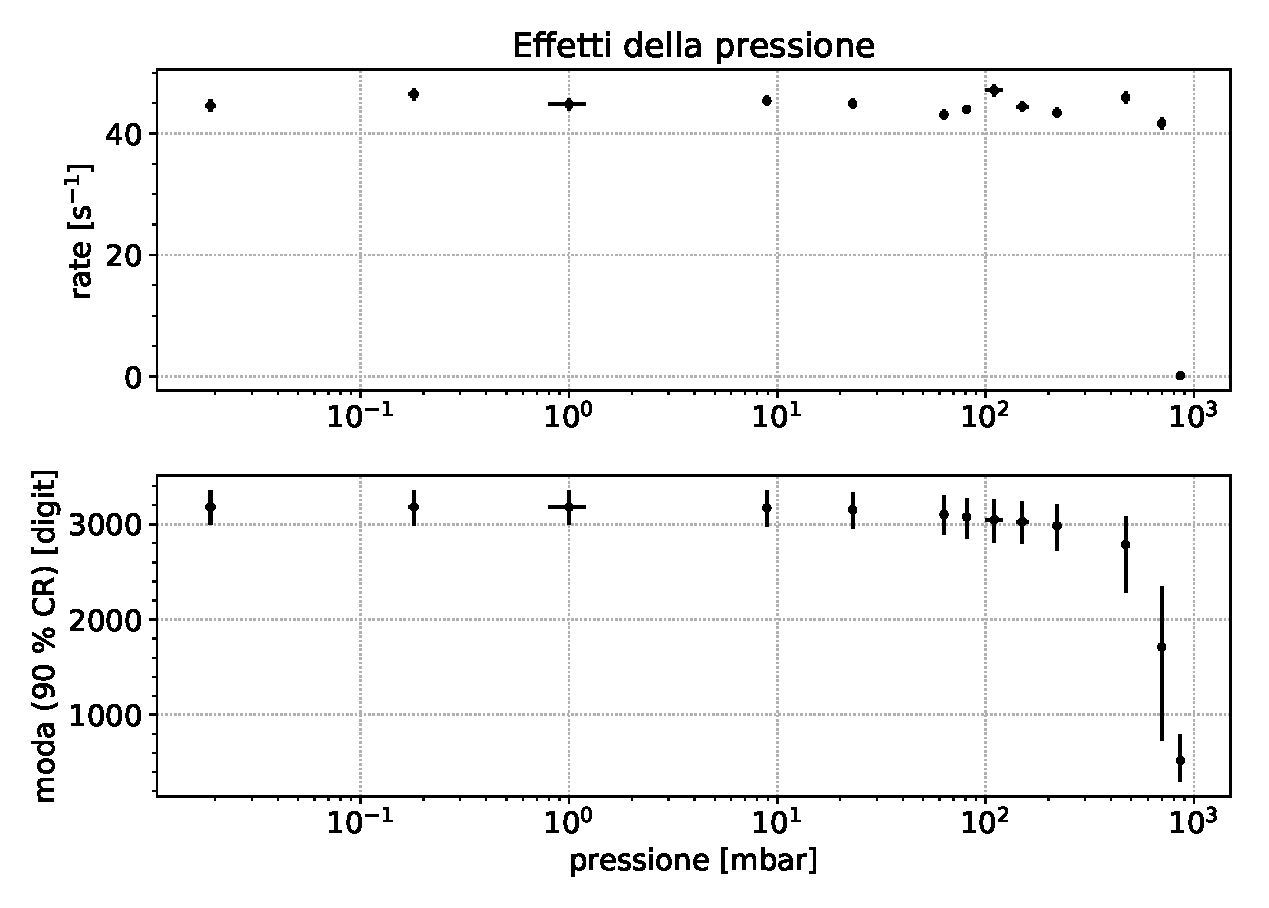
\includegraphics[width=30 em]{immagini/press}
\caption{Effetti della pressione su conteggi e spettri. Il pannello superiore mostra il variare del rate al variare la pressione, quello sottostante contiene la moda dei relativi spettri con errore un intervallo del 90\% di credibilità.}
\label{fig:press}
\end{figure}

\marginpar{Il 90\% di credibilità mi sembra eccessivo come errore. Si vedono i punti che scendono, ma gli errori enormi fanno credere che sia tutto compatibile. 
Ho guardato gli spettri e mi sono accorto che, alzando la pressione, le distro si allargano. Me ne farò una ragione.}

Dal grafico di \autoref{fig:press} non si nota nessuna variazione dei conteggi fino ad \SI{1}{atm}, ma la moda dello spettro inizia a decrescere quando la pressione è maggiore di \SI{200}{mbar}. 
Come atteso, la distribuzione di energia persa dalle particelle $\alpha$ in aria diventa sempre più larga all'aumentare della pressione.
Questo risultato ci assicura una grande indipendenza dalla condizione di vuoto della camera. 
\marginpar{aggiungere questione misure notturne}

\marginpar{secondo me dobbiamo mostrare questa cosa con l'istogramma di alcuni spettri perché dà un'idea più immediata rispetto al fornire l'intervallo di credibilità}